\FloatBarrier
\section{}
% Question 2 Reconsider the closed-loop diagram from Question 1, now with
% Gc(s) = 2 + 2
% s
% , Gp(s) = 1
% s − 1
% i.e. a BIBO unstable plant connected to a PI controller.
% (a) By hand, sketch the Nyquist contour D and Nyquist plot G, then apply Theorem 5.3.1 to
% check the stability of the closed-loop system
% (b) Give the plot obtained with MATLAB’s nyquist command. What’s the major difference
% between this result and the sketch from (a)?

Reconsider the closed-loop diagram from Question 1, now with
\begin{equation*}
    G_c(s) = 2 + \frac{2}{s}=\frac{2s + 2}{s}, \quad G_p(s) = \frac{1}{s-1}
\end{equation*}
i.e. a BIBO unstable plant connected to a PI controller.
\begin{enumerate}[label=(\alph*)]
    \item By hand, sketch the Nyquist contour $\mathcal{D}$ and Nyquist plot $\mathcal{G}$, then apply Theorem 5.3.1 to
    check the stability of the closed-loop system
    \item Give the plot obtained with MATLAB's \texttt{nyquist} command. What's the major difference
    between this result and the sketch from (a)?
\end{enumerate}

\subsection{}
The loop transfer function $L(s)$ is given by
\begin{equation*}
    L(s) = G_p(s)G_c(s) = \frac{2s + 2}{s(s-1)}
\end{equation*}
The poles are at $s=0$ and $s=1$. Since there is a pole at $s=0$, a small semi-circle of radius $\epsilon$ is drawn
around the origin. 

From $a$ to $b$, $s = j \omega$, $\omega \in [0, \infty)$,
\begin{align*}
    L(j \omega) &= \frac{2j \omega + 2}{j \omega (j \omega - 1)} \\
\end{align*}
With help from MATLAB, 
\begin{lstlisting}[language=Matlab]
syms s omega real
L(s) = (2*s + 2)/(s*(s-1));
simplify(real(L(j*omega)))
simplify(imag(L(j*omega)))
\end{lstlisting}
which gives
\begin{equation*}
    \text{Re} \left\{ L(j \omega) \right\} = \frac{-4}{\omega^2 + 1}, \quad \text{Im} \left\{ L(j \omega) \right\} = \frac{2 (1 - \omega^2)}{\omega (\omega^2 + 1)}
\end{equation*}
Starting at point $a$ the point $s = j \epsilon$, 
\begin{equation*}
    \text{Re} \left\{ L(j \epsilon) \right\} = \frac{-4}{\epsilon^2 + 1} \approx -4, \quad \text{Im} \left\{ L(j \epsilon) \right\} 
    = \frac{2 (1 - \epsilon^2)}{\epsilon (\epsilon^2 + 1)} \to \infty
\end{equation*}
to point $b$, $s = j \omega$, $\omega \to \infty$,
\begin{equation*}
    \text{Re} \left\{ L(j \omega) \right\} = \frac{-4}{\omega^2 + 1} \to 0, \quad \text{Im} \left\{ L(j \omega) \right\} 
    = \frac{2 (1 - \omega^2)}{\omega (\omega^2 + 1)} \to 0
\end{equation*}
By symmetry, $c$ to $d$ is the same as $a$ to $b$ reflected about the real axis. Note the curve intersects the real axis at $s = -2$ on its 
way to $b$ and $c$.

The last section $a$ to $d$ is derived in the notes as 
\begin{equation*}
    L(\epsilon e^{j \theta}) \approx \frac{e^{-j \theta}}{\epsilon} \frac{2s + 2}{s-1}
\end{equation*}
which sweeps out a semi-circle of infinite radius of angular distance $\pi$. 

The Nyquist plot is shown in Figure \ref{fig:Q2Sketch}
\begin{figure}[h]
    \centering
    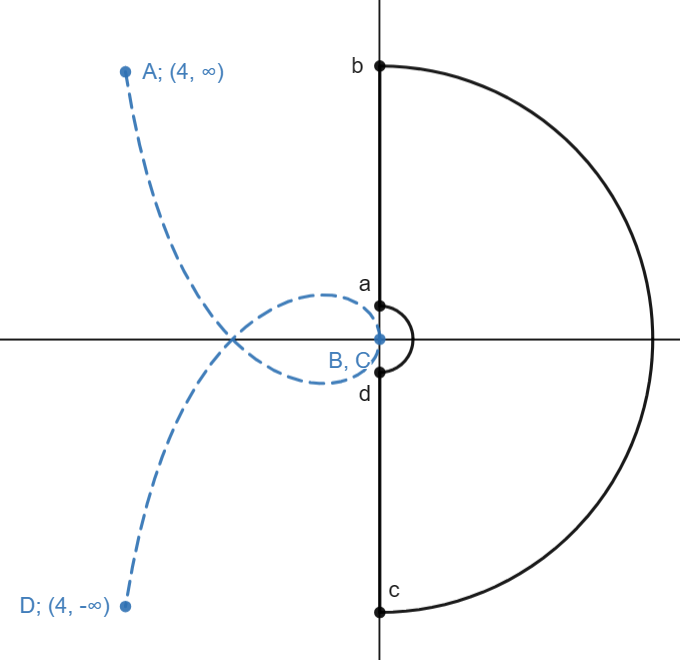
\includegraphics[width=0.3\textwidth]{Questions/Figures/Q2Sketch.png}
    \caption{2(a) Nyquist sketch}
    \label{fig:Q2Sketch}
\end{figure}

Since there is one pole Re$(s) > 0$, $n = 1$. Since the Nyquist plot does not pass through $-1$ and encircles it once in the counter-clockwise direction,
the closed-loop system is stable.

\subsection{}
\begin{lstlisting}[language=Matlab]
nyquist(tf([2 2], [1 -1 0]))
\end{lstlisting}
\begin{figure}[h]
    \centering
    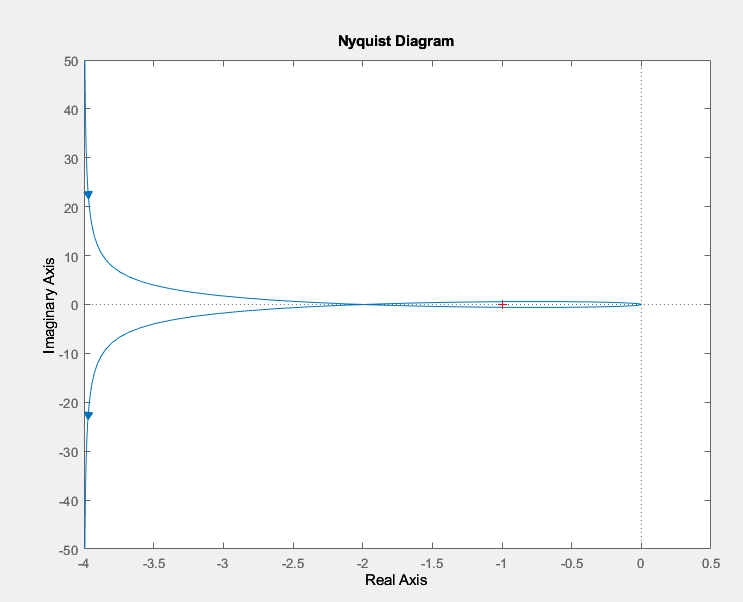
\includegraphics[width=0.5\textwidth]{Questions/Figures/Q2Matlab.png}
    \caption{2(b) Nyquist plot generated by MATLAB}
\end{figure}

The major difference is the lack of the semi-circle of infinite radius. The sketch approximated the infinite radius semi-circle as a
semi-circle of finite radius.

